\documentclass[11pt, 
%oneside, % Two side (alternating margins) for binding by default, uncomment to switch to one side
ngerman,
%singlespacing, % Single line spacing, alternatives: 
%onehalfspacing,
%or 
doublespacing,
%draft, % Uncomment to enable draft mode (no pictures, no links, overfull hboxes indicated)
%nolistspacing, % If the document is onehalfspacing or doublespacing, uncomment this to set spacing in lists to single
%liststotoc, % Uncomment to add the list of figures/tables/etc to the table of contents
%toctotoc, % Uncomment to add the main table of contents to the table of contents
%parskip, % Uncomment to add space between paragraphs
%nohyperref, % Uncomment to not load the hyperref package
%headsepline, % Uncomment to get a line under the header
chapterinoneline, % Uncomment to place the chapter title next to the number on one line
consistentlayout, % Uncomment to change the layout of the declaration, abstract and acknowledgements pages to match the default layout
]{scrartcl}
\usepackage{ngerman}
\usepackage{graphicx}
\usepackage{hyperref} 
\usepackage[figure]{hypcap}
\usepackage{url}

\newtheorem{definition}{Definition}

\begin{document}
\author{Niels Gundermann}
\title{Kommunikation zwischen entkoppelten Java-Modulen über strukturell typkonforme Objekte

%Verwendung strukturell typkonformer Java-Objekte in voneinander entkoppelten Modulen 
}
\maketitle
\section{Einleitung}
Die Modularisierung ist ein gängiges Mittel zur Beherrschung komplexer Softwaresys\-teme. Die Kommunikation zweier Module wird dabei durch eine vorab definierte Schnitt\-stelle gewährleistet. Bei der Kommunikation kann es sich lediglich um den Aufruf eines Dienstes handeln, oder um einen Datenaus\-tausch über so genannte Transfer-Objekte.\\\\
In der Programmiersprache Java wer\-den diese Schnittstellen im Allgemeinen häufig als Interfaces definiert und gliedern sich somit in die Typ-Hierarchie des Programms ein. Soll ein Modul \emph{A} mit einem Modul \emph{B}  kommunizieren, so müssen beide Module ein Interface \emph{I} als Schnittstelle kennen und sind damit abhängig von diesem. Wenn es zu einem Datenaustausch über \emph{I} kommen soll, so müssen die beiden Module darüber hinaus die Typen kennen, durch die die Transfer-Objekte abgebildet werden (Transfer-Typen).\\\\
Die Konformität der Typen (Transfer-Typen und Interfaces) wird in Java auf nominaler Ebene, also auf der Basis der Bezeichnung des jeweiligen Typs, sichergestellt (Nominale Typkonformität).
Die dadurch entstehende Abhängigkeit führt zu einer Behinderung möglicher paralleler Arbeiten an diesen Modulen - insbesondere dann, wenn die Schnitt\-stelle im Zuge der Arbeiten angepasst werden muss und die beiden Module im Verantwor\-tungs\-bereich unterschiedlicher Entwicklerteams liegen.\\\\ 
Ein anderer Ansatz zur Sicherstellung der Typkonformität beruht auf dem Abgleich der strukturellen Eigenschaften von Typen (Strukturelle Typkonformität). Dabei werden die Transfer-Typen und Interfaces, die für die Kommunikation zwischen zwei Modulen (\emph{A} und \emph{B}) benötigt werden, innerhalb beider Module definiert, sodass jedes Modul seine eigenen Typen bereitstellt. Die beiden Module wären somit voneinander und von einer gemeinsamen Schnitt\-stelle (\emph{I}) syntaktisch unabhängig.
%, da die Konformität zwischen den Typen, nicht anhand der Bezeichnung gewährleistet wird, sondern auf der Basis  gleicher Strukturen der in beiden Modulen definierten Interfaces und Transfer-Typen für die jeweilige Kommunikation.
\\\\
Es gab bereits Überlegungen dazu, wie eine strukturelle Typkonformität in der Program\-mier\-sprache Java umgesetzt werden könnte (vgl. \cite{whiteoak}, \cite{structconfjava}). Die Arbeit von Läufer et al. (\cite{structconfjava}) beschränkt sich dabei jedoch nur auf die Konformität zwischen Klassen und Interfaces und bedingt eine Anpasssung des Java-Compilers. Bei der Lösung von Gil et al. (\cite{whiteoak}) handelt es sich um eine Spracherweiterung, was die Integration in bestehende Systeme erheblich erschwert.
% Die dafür notwendigen Erweiterung beschränkten sich jedoch nur auf die Konformität zwischen Klassen und Interfaces (vgl. \cite{structconfjava}) oder erfordern eine Spracherweiterung (vgl. \cite{whiteoak}).
\\\\ 
Die vorliegende Arbeit befasst sich mit einem Ansatz der einerseits als Java-Bibliothek integriert werden kann und andererseits auch die Konformität zwischen Klassen als Transfer-Typen herstellen soll. 
Aufgrund der Tatsache, dass die Methoden strukturell typkonformer Objekte, in unterschiedlichen Modulen auch unterschiedlich implementiert werden können, muss entschieden werden, welche der Implementierung letztendlich ver\-wendet werden soll. Auf dieses Problem wird ein besonderer Fokus innerhalb dieser Arbeit gelegt.
Dies betrifft natürlich nicht nur Methoden-Implementierungen in Klassen, sondern auch default-Methoden in Interfaces.

\subsection{Problembeschreibung}\label{problembeschreibung}
In dieser Arbeit werden zwei Szenaien betrachtet, die unterschiedliche Probleme aufzeigen. In beiden Fällen wird ein Ausschnitt aus einem System beschrieben, dessen Aufbau den Prinzipien einer strengen Schichtenarchitektur folgt  (siehe \ref{architektur}).
\subsubsection{Szenario 1}\label{prob1}
Auf architektonischer Ebene kann das erste Szenario, wie im Abbildung \ref{fig:problem} folgt dargestellt werden.
\begin{figure}[h]
  \centering
  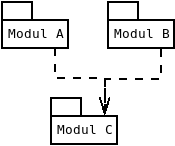
\includegraphics[scale = 0.7]{pics/problemS1Abstrakt.png}
  \caption{Problem: Szenario 1 (abstrakt)}
  \label{fig:problem}
\end{figure}
Die Module \emph{A} und \emph{B} liegen architektonisch auf der gleichen Ebene und dürfen somit keine direkte Abhängigkeiten aufweisen. Das Modul \emph{C} stellt eine Abstraktionsebene dar, die für das gesamte System verwendet wird. Änderungen an diesem Modul würden demnach nicht nur die Module \emph{A} und \emph{B} betreffen, sondern auch noch weitere Module, die in Abbildung \ref{fig:problem} nicht aufgeführt sind. Zudem soll zusätzlich davon ausgegangen werden, dass die Module \emph{A} und \emph{B} im Verantwortungsbereich eines Eintwicklerteams \emph{E1} liegen, während das Modul \emph{C} im Verantwortungsbereich eines Entwicklerteams \emph{E2} liegt.\\\\
Ein konkretes Beispiel hierzu ist in Abbildung \ref{fig:problem1Konkret} zu sehen.
\begin{figure}[h]
  \centering
  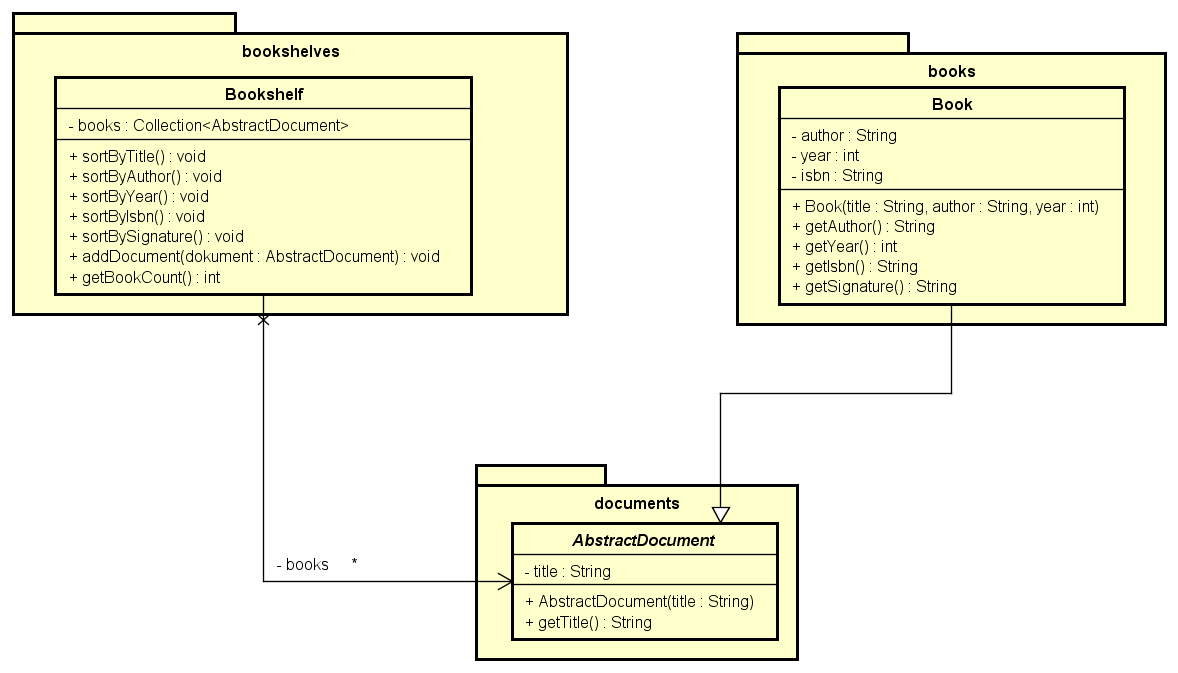
\includegraphics[scale = 0.3]{pics/problemS1Konkret.png}
  \caption{Problem: Szenario 1}
  \label{fig:problem1Konkret}
\end{figure}\\
Hier liegen die Module \emph{bookshelves} und \emph{books} auf einer Architekturebene, analog zu den abstrakten Modulen \emph{A} und \emph{B}. Dementsprechend stellt das Modul \emph{documents} das Pendant zum abstrakten Modul \emph{C} dar. Zu erkennen ist, dass die Klasse \emph{Bookshelf} im Modul \emph{bookshelves} einige Sortier-Methoden enthält. Da die Klasse \emph{AbstractDocument} aus dem Modul \emph{documents} jedoch lediglich einen \emph{title} enthält, wäre die Implementierung eines Algorithmus zur Sortierung nach dem Jahr (\emph{sortByYear}) oder nach dem Autor (\emph{sortByAuthor}) nur schwer umzusetzen. Würde hingegen die Klasse \emph{Book} aus dem Modul \emph{books} in der Klasse \emph{Bookshelf} nutzbar sein, könnten der Entwickler das \emph{year} und den \emph{author} bei der Implementierung der Sortier-Algorithmen verwenden.\\\\
%Nun wird eine abstrakte Klasse aus Modul \emph{C} in Modul \emph{B} konkret implementiert. Weiterhin werden Objekte, die in Modul \emph{B} erzeugt werden in Modul \emph{A} verwendet. Die Verwendung erfolgt jedoch über die abstrakte Klassendefinition aus Modul \emph{C}.\\\\
%Aufgrund einer geänderten Anforderung muss innerhalb von Modul \emph{A} eine Information genutzt werden, die bereits in der konkreten Implementierung aus Modul \emph{B} vorliegt, aber nicht in der abstrakten Implementierung aus Modul \emph{C} zur Verfügung steht. In diesem Szenario gäbe es aufgrund der nominalen Typkonformität folgenden Lösungsvarianten:
Aufgrund der nominalen Typkonformität gäbe es für dieses Szenario folgende Lösungsvarianten:
\begin{enumerate}
\item Die abstrakte Impementierung wird um diese Information erweitert.
\item Es wird eine weitere Abstraktionsschicht zwischen den beiden vorliegenden Schichten eingebaut.
\end{enumerate}
Beide Lösungsvarianten führen zu relativ hohem Anpassungsaufwand, wenn man bedenkt, dass die benötigte Information bereits zur Verfügung steht.
\subsubsection{Szenario 2}\label{prob2}
Das zweite Szenario bezieht sich auf eine Serviceorientierte Architektur (siehe \ref{sarchitektur}).
Abbildung \ref{fig:problem2} zeigt den angenommenen Ausschnitt aus einem System. 
\begin{figure}[h]
  \centering
  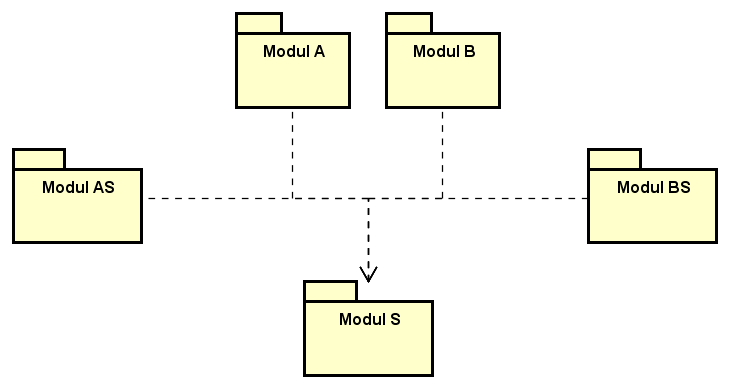
\includegraphics[scale=0.7]{pics/problemS2Abstrakt.png}
  \caption{Problem: Szenario 2}
  \label{fig:problem2}
\end{figure}\\
Hierbei wird von einem Broadcast Serviceaufruf ausgegangen. Sas bedeutet, dass es eine Service-Schittstelle gibt, die in mehreren Modulen implementiert wird. Die Aufrufer liegen in diesem Fall in Modul \emph{A} und \emph{B}, während die Service-Schnittstelle in Modul \emph{S} liegt. Die weiteren Module beinhalten unterschiedliche Implementierungen des augerufenen Services. Weiterhin ist anzunehmen, dass alle Module im Verantwortungsbereich unterschiedlicher Entwicklerteams liegen.\\\\
Abbildung \ref{fig:problem2Konkret} zeigt ein konkretes Beispiel für dieses Szenario.
\begin{figure}[h]
  \centering
  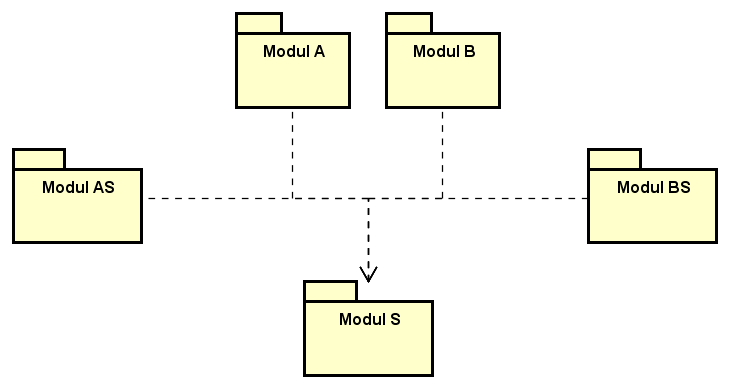
\includegraphics[scale=0.7]{pics/problemS2Abstrakt.png}
  \caption{Problem: Szenario 2}
  \label{fig:problem2Konkret}
\end{figure}\\
Im Speziellen ist hier eine Art Notruf-Szenario abgebildet. Dabei gibt es ein Modul \emph{injured}, in dem unterschiedliche Personen, die sich verletzen können bzw. in eine Notsituation geraten könnten, über die Klassen \emph{Person} und \emph{Allergic} abgebildet sind. Die daraus entstehenden Objekte können über einen Service aus dem Modul \emph{MedicalServices} medizinische Hilfe anfordern. Die konkreten Services werden in den Modulen \emph{doctors} und \emph{cardriver} bereitgestellt. (Fachlich gesehen handelt es sich bei den Services also um eine Art Erstversorgung bzw. Erste-Hilfe).\\\\
Nun ist aber davon auszugehen, dass ein Allergiker (\emph{Allergic}) mitunter eine andere medizinische Erstversorgung benötigt, als eine Person, die keine Allergien aufweist (\emph{Person}). Weiterhin wäre vorstellbar, dass der Allergiker spezielle Informationen oder Werkzeuge, die für die notwendige Versorgung benötigt werden, bei sich trägt. (Beispielsweise einen Notimpfstoff mit Instruktionen zur Verabreichung.) Um diese zusätzlichen Informationen in den Service-Implementierungen nutzen zu können, gäbe es basierend auf der Tatsache, dass eine nominale Typkonformität im System angenommen wird, folgende Lösungsansätze:
%Nun ist davon auszugehen, dass innerhalb von Modul \emph{A} eine weitere Information durch den Service bereitgestelt werden soll. Hierbei gibt es folgende Lösungsansätze:
\begin{enumerate}
\item Die Service-Schnittstelle wird erweitert.
\item Es wird eine neue Service-Schnittstelle geschaffen, die auf die zusätzlichen Informationen Zugriff hat.
\end{enumerate}
Beide Lösungsansätze erfordern wiederrum erheblichen Aufwand und Koordination zwischen den Entwicklerteams. Dabei ist zu erwähnen, dass der zweite Lösungsansätz etwas weniger Aufwand erfordert, da die Entwicklerteams, deren Service-Implementierungen ohnehin in Modul \emph{A} keine Verwendung finden, nicht beteiligt sind. 

\section{Typen und Typkonformität}
\cite{types}
\subsection{Typen in Java}
\subsection{Typkonformität in Java}
\cite{structconfjava}, \cite{compoundtypes}
\subsection{Zufällige Typkonformität}
\cite{structconfjava}
\section{Softwarearchitektur}
\cite{Bas13}
\subsection{Schichtenarchitektur}\label{architektur}
\cite{modanwendungen}
\subsection{Serviceorientierte Architektur}\label{sarchitektur}
\cite{modanwendungen}
\subsection{Schnittstellen}
\cite{Bas13}, \cite{Bus96}
\section{Lösungsansätze}
%\subsection{Bestehende Lösungen}
In den folgenden Kapiteln wird auf die Lösungsmöglichkeiten der in \ref{problembeschreibung} beschriebenen Szenarien mit den bestehenden Lösungen nach \cite{structconfjava} und \cite{whiteoak} eingegangen. Die hier beschriebenen Lösungsansätze basieren lediglich auf den theoretischen Ausführungen bzgl. der allgemeinen Ansätze. Es wurde kein praktischer Nachweis in Form einer Implementierung erbracht, der die theoretischen Grundlagen aus \cite{structconfjava} und \cite{whiteoak} bestätigt. Das Ziel dieses Abschnittes der Arbeit ist es, grundlegende Konzepte, die in den nachfolgenden Lösungsansätzen enthalten sind, aufzunehmen und weiterzuentwickeln.
\subsection{Erweitung des Java-Compilers}
In der Arbeit von Läufer et. al. (\cite{structconfjava}) wurde der Java-Compiler so erweitert, dass die Deklaration der implementierten Interfaces an einer Klasse entfallen kann. Die Substituierbarkeit nach dem eines Interfaces und einer Klasse nach dem Liskovschen Substitutionsprinzip wird durch den Java-Compiler zusätzlich auf Basis der Struktur der entsprechenden Klassen und Interfaces festgestellt.\\\\
Hierzu musste definiert werden, was unter Typkonformität innerhalb der Sprache Java zu verstehen ist. Dabei wurden beachtet, dass in Java sowohl Klassen als auch Interfaces als Typen fungieren. Allgemein wurde folgende formale Definition hinsichtlich der Typkonformität aufgestellt:
\begin{definition}\label{def_allgTypkonfJava}
Sei \emph{I} ein Interface und \emph{X} sowie \emph{Y} jeweils eine Klasse oder ein Interface.\\
In der Sprache Java hat jede Klasse mit Außnahme von \emph{java.lang.Object} eine direkte Oberklasse. Jede Klasse und jedes Interfaces hat keine ider mehrere direkte Interfaces.\\\\
\emph{X} ist konform zu \emph{Y} genau dann, wenn:
\begin{itemize}
\item\emph{X} nominal Typkonform zu \emph{Y} ist, oder
\item\emph{Y} ein Interface ist, das strukturelle Typkonformität erlaubt und zu \emph{X} strukturell Typkonform ist.
\end{itemize}
\end{definition} (vgl. \cite{structconfjava}) \\\\
An Definition \ref{def_allgTypkonfJava} ist zu erkennen, dass die nominale Typkonformität in dem Ansatz von Läufer et. al \cite{structconfjava} nicht ausgeschlossen wurde, sodass die Konformität zweier Typen sowohl auf nominaler als auch struktureller Ebenen definiert ist. Die nominale Typkonformität wird in diesem Ansatz dabei wie folgt definiert:
\begin{definition}
\emph{X} ist nominal typkonform zu \emph{Y} genau dann, wenn:
\begin{itemize}
\item \emph{X} ist identisch zu \emph{Y}, oder
\item die direkte Oberklasse von \emph{X}, sofern sie existiert, ist nominal typkonform zu \emph{Y}, oder
\item ein direktes Interface \emph{I} von \emph{X} ist nominal typkonform zu \emph{Y}
\end{itemize}
\end{definition} (vgl. \cite{structconfjava})\\\\
Die strukturelle Typkonformität wird in dem Ansatz aus \cite{structconfjava} wie folgt definiert:
\begin{definition}\label{def_structTypkonfJava}
\emph{X} ist strutkurell typkonform zu \emph{I} genau dann, wenn \emph{X} nominal typkonform zu \emph{I} ist, oder alle der folgenden Bedingungen gleichzeitig erfüllt sind:
\begin{itemize}
\item \emph{I} ist ein Interface, dass strutkurelle Typkonformität erlaubt, und
\item \emph{X} überschreibt jede Methode, die in \emph{I} spezifiziert ist, und
\item \emph{X} ist typkonform zu allen direkten Interfaces von \emph{I}.
\end{itemize}
\end{definition} (vgl. \cite{structconfjava})\\\\
Zur Vollständigkeit der Definitionen muss weiterhin definiet werden, wann eine Methode eines Interfaces in einer Klasse oder Interface überschrieben wird. Das Überschreiben einer Methode wird dabei wie folgt definiert:
\begin{definition}\label{def_override}
\emph{X} überschreibt eine Methode \emph{Y.f}, die in \emph{Y} spezifiziert ist, genau dann, wenn es eine Methode \emph{f} in \emph{X} gibt (\emph{X.f}), die folgende Bedingungen erfüllt:
\begin{itemize}
\item \emph{X.f} ist von der Sichtbarkeit her nicht stärker eingeschränkt als \emph{Y.f}.
\item \emph{X.f} hat dieselbe Methodensignatur wie \emph{Y.f}
\item Checked Exceptions, die von \emph{X.f} geworfen werden, sind Unterklassen oder von derselben Klasse, die auch der Checked Excpetions zugrundeliegen, die von \emph{Y.f} geworden werden.
\end{itemize}
\end{definition} (vgl. \cite{structconfjava})\\\\
Da der Ansatz aus \cite{structconfjava} eine Hybride Variante bzgl. der Feststellung der Typkonformität darstellt (Verwendung von nominaler und struktureller Typkonformität) musste festgelegt werden, welche From der Typkonformität als Standardvariante verwendet wird. Anderenfalls würde die Gefahr der \emph{versehentlichen Typkonformität} bestehen. Aufgrunddessen wurde festgelegt, dass die nominale Typkonformität als Standardvariante verwendet wird und die strukturelle Typkonformität einer speziellen Erlaubnis bedarf. (vgl. \cite{structconfjava}) Dieser Fakt ebenfalls bei genauerer Betrachtung der Definitionen \ref{def_allgTypkonfJava} und \ref{def_structTypkonfJava} klar. In diesen Definitionen ist die Rede davon, dass ein Interface die strukturelle Typkonformität erlaubt. Wann ein Interfaces die sturkutrelle Typkonformität erlaubt, ist in Definition \ref{def_allowStruct} festgehalten: \begin{definition}\label{def_allowStruct}
Ein Interface erlaubt die sturkturelle Typkonformität, wenn eine der folgenden Bedingungen erfüllt ist:
\begin{enumerate}
\item Das Interface erweitert ein speziellen Marker-Interface (z.B. \emph{Structural})
\item Das Interface erweitert ein anderes Interface, welches strukturelle Typkonformität erlaubt
\end{enumerate} 
\end{definition} (vgl. \cite{structconfjava})\\\\
Ausgehend von den Definitionen \ref{def_allgTypkonfJava} - \ref{def_allowStruct} können die beiden Problem-Szenarien aus Kapitel \ref{problembeschreibung} wie folgt mithifle dieses Ansatzes umgesetzt werden:





\subsection{WHITEOAK}
\cite{whiteoak}
%\subsubsection{REST/SOAP}
\\\\
\subsection{Neuer Lösungsansatz}
In den folgenden Kapiteln wird auf die Umsetzung der Problem-Szenarien aus Kapitel \ref{problembeschreibung} unter der Verwendung des im Rahmen dieser Arbeit erarbeiteten Ansatz beschrieben.\\\\
Dieser Lösungsansatz verwendet weder einen erweiterten Compiler noch eine Erweiterung der Sprachekonstrukte. Die Verwendung der strukturellen Typkonformität muss innerhalb der Programms mithilfe einer einzubindenden Bibliothek explitit angestoßen werden. Hierzu steht in der Bibliothek das Interface \emph{TypConverter} bereit, welches die Verwendung der strukturellen Typkonformität ermöglicht. Ein Objekt, welches das Interfaces \emph{TypConverter}  erfüllt, kann mithilfe der Klasse \emph{TypConverterBuilder} erzeugt werden. Auf die Parameter, die dem \emph{TypConverterBuilder} mitgegeben werden müssen, wird im späteren Verlauf spezieller eingegangen. Im Allgemeinen dienen sie der Konfiguration der Konformitätsprüfung sowie der Form Konvertierung von strukturell typkonformen Objekten.\\\\
Der neue Lösungsansatz geht über den Ansatz von Läufer et. al \cite{structconfjava} insofern hinaus, dass sich eine strukturelle Typkonformität nicht nur zwischen Klassen und Interfaces feststellen lässt, sondern auch zwischen zwei Klassen. 



\subsection{Interfaces als Schnittstellen-Typ}
Im ersten Teil wird beschrieben, wie mit Interfaces als sturkturelle Typen umgegangen wird. Da Läufer et. al. \cite{structconfjava} in ihrer Arbeit hierfür bereits eine fundierte Grundlage geschaffen haben, werden die Definitionen \ref{def_allgTypkonfJava} - \ref{def_override} auch als theoretische Grundlage für den neuen Lösungsansatz verwendet.\\\\
Da die Verwendung der strukturellen Typkonformität im neuen Lösungsanstz explizit angegeben werden muss, ist es anders als im Ansatz aus \cite{structconfjava} nicht notwendig, die Interfaces, für die eine sturkturelle Typkonformität Anwendung finden kann, explizit durch Marker-Interfaces zu markieren. Folglich wird die Definition \ref{def_allowStruct} für den neuen Lösungsansatz nicht benötigt. Ausgehen davon kann auch die Definitionen \ref{def_allowStruct} und \ref{def_structTypkonfJava} für den neuen Lösungsansatz nicht verwendet werden. Allerdings sind nur kleinere folgende Anpassungen notwendig, um Definitionen für die Verwendungen der strukturellen Typkonformität in Bezug auf  Interfaces nach dem neuen Lösungsansatz als Basis zu formulieren.
\begin{definition}\label{def_allgTypkonfJava_V1}
Sei \emph{I} ein Interface und \emph{X} sowie \emph{Y} jeweils eine Klasse oder ein Interface.\\
In der Sprache Java hat jede Klasse mit Außnahme von \emph{java.lang.Object} eine direkte Oberklasse. Jede Klasse und jedes Interfaces hat keine oder mehrere direkte Interfaces.\\\\
\emph{X} ist konform zu \emph{Y} genau dann, wenn:
\begin{itemize}
\item\emph{X} nominal Typkonform zu \emph{Y} ist, oder
\item\emph{Y} ein Interface ist, das zu \emph{X} strukturell Typkonform ist.
\end{itemize}
\end{definition}
\begin{definition}\label{def_structTypkonfJava_V1}
\emph{X} ist strutkurell typkonform zu \emph{I} genau dann, wenn \emph{X} nominal typkonform zu \emph{I} ist, oder alle der folgenden Bedingungen gleichzeitig erfüllt sind:
\begin{itemize}
\item \emph{X} enthält für jede Methode, die in \emph{I} spezifiziert ist, eine strukturell äquivalente Methode und
\item \emph{X} ist typkonform zu allen direkten Interfaces von \emph{I}.
\end{itemize}
\end{definition} (vgl. \cite{structconfjava})
\begin{definition}\label{def_containMethod_V1}
\emph{X} enthält eine Methode \emph{f} (\emph{X.f)}, die strukturell äquivalenz zu einer Methode \emph{Y.f} ist, wenn \emph{X.f} \emph{Y.f} lauf Definition \ref{def_override} überschreibt, oder alle der folgenden Bedingungen erfüllt sind:
\begin{itemize}
\item \emph{X.f} ist von der Sichtbarkeit her nicht stärker eingeschränkt als \emph{Y.f}
\item \emph{X.f} hat denselben Rückgabetyp wie \emph{Y.f}
\item \emph{X.f} benötigt dieselben Parameter in derselben Reihenfolge wie \emph{Y.f}
\item Checked Exceptions, die von \emph{Y.f} geworden werden, werden auch von \emph{X.f} geworfen, wobei diese in \emph{X.f} auch als Unterklassen derer, die von \emph{Y.f} geworden werden, umgesetzt sein können
\end{itemize} 
\end{definition}
Diese Grundlage unterscheiden sich wie folgt von derer aus dem Ansatz von Läufer et. al. \cite{structconfjava} wie folgt. Zum einen ist es nicht mehr notwendig, dass ein Interface die strukturelle Typkonformität erlauben muss, um eine strutkurelle Typkonformität zu gewähleisten. Weiterhin können sich die Methoden zweier strukturell konformer Typen durchaus vom Namen her unterscheiden. Die Definition \ref{def_containMethod_V1} erlaubt dabei zwei Wege, um das \emph{Enthalten} einer strukturell äquivalenten Methode in einer Klasse zu gewährleisten. Der erste Weg besteht im Überschreiben der Methode gemät Defintion \ref{def_override}. Der zweite Weg fordert hingegen nicht, dass die Bezeichnungen der Methoden gleich sein müssen. Diese Herangehensweise kann jedoch zu Problemen führen. So kann die strukturelle Typkonformität zwischen einem Interface und einer Klasse, wie in Abbildung \ref{ambigousStructMethods}, zwar festgestellt werden. Eine Konvertierung und damit Nutzung des Konzepts ist aber nicht möglich. 
%\begin{figure}[h]
%\includegraphics[]{}
%\label{ambigousStructMethods}
%\end{figure} 
Die Klasse ist auf Basis der o.g. Definitionen strukturell Typkonform zum Interface. Bei der Konvertierung muss jedoch festgestellt werden, welche Methode innerhalb der Klasse das strukturelle Äquivalent zur Methode aus dem Interface darstellt. Da die Methodensignaturen abgesehen vom Methodennamen aller Methoden gleich sind, sind auch alle Methoden sturkturell äquivalent.\\\\
Für dieses Problem wurde im \emph{TypConverterBuilder} die Möglichkeit geschaffen, einen der beiden Wege zur Ermittlung der strukturell äquivalenten Methoden explizit anzugeben. So kann der Entwickler selbst entscheiden, welchen Ansatz er verwendet und muss in der Konsequenz die Klassen und Interfaces bzgl. der Methoden dementsprechen so entwerfen, dass der gewünschte Ansatz verwendet werden kann.\\\\
Daher muss beim Erzeugen eines Objekte vom \emph{TypConverterBuilder} eine \emph{ComformityCheckingBase} angegeben. Diese kann genau zwei Werte annehmen, wobei der erste (\emph{Name}) die Ermittlung der strukturell äquivalenten Methoden nach Definition \ref{def_override} angibt und die zweite (\emph{SIGNATURE}) die Ermittlung auf Basis der Signatur, als ohne Beachtung des Methodennamens, angibt.
%In Abhängigkeit werden unterschiedliche TypConverter erzeugt
\\\\
Bezogen auf das erste Problemszenario (siehe Kapitel \ref{prob1}) sähe eine Lösungsvariante über ein strukturell typkonformes Interfaces wie folgt aus. Der Typ, der in dem Modul \emph{Bookshelves} die Elemente abbilden soll, die innerhalb der Objekte der Klasse \emph{Bookshelf} verwaltet werden, könnte innerhalb des Moduls, wie in Abbildung \ref{solveInterface_PS1} spezifiziert werden.
\begin{figure}[h]
%\includegraphics[draft]{foo}
\caption{Lösungsansatz: Interfaces - Problemszenario 1}
\label{solveInterface_PS1}
\end{figure} 
Hierbei ist zu bemerken, dass es sich bei den Methoden im Interface \emph{BookForBookshelf} um genau die Methoden handelt, die in den Sortier-Methoden der Klasse \emph{Bookshelf} Verwendung finden. Bei genauerer Betrachtung der Klasse \emph{Book} aus dem Modul \emph{Books} fällt auf, dass diese Klasse strukturell typkonform zu dem neune Interface \emph{BookForBookshelf} ist. Die Frage die offen bleibt ist, wie ein Objekt der Klasse \emph{Book} in ein Objekt vom Typ \emph{BookForBookshelf} konvertiert wird.\\\\
Grundsätzlich kann die Konvertierung in diesem Fall nur im Modul \emph{Bookshelves} stattfinden, da nur dort der Zugriff auf den \emph{Ziel-Typ} - in diesem Fall \emph{BookForBookshelf} - gewährleistet ist. Zu bemerken ist, dass innerhalb den Moduls zwar ein Objekt der Klasse \emph{Book} zu verwenden ist, der konkrete Typ des Objektes jedoch für das Einleiten der Konvertierung irrelevant ist. Somit kann zur Not das konkrete Objekt einer Klasse aus einem anderen Modul - wie in diesem Fall \emph{Book} aus dem Modul \emph{Books} - mit dem Typ \emph{java.lang.Object} verwendet werden. In diesem speziellen Fall wäre es jedoch von Vorteil, die bestehende Signatur der Methode zum Hinzufügen von Elementen in ein \emph{Bookshelf} beizubehalten, da der dort benötigte Typ aus einer Abstraktionsebene stammt, auf die beide Module - \emph{Books} und \emph{Bookshelves} - zugreifen dürfen. Somit können die Methoden der Klasse \emph{Bookshelf} von der Signatur her für diesen Lösungsweg unverändert bleiben, was den Entscheidenen Vorteil mit sich bringt, dass die verwendenen Klassen nicht angepasst werden müssen.\\\\
Der Entwickler muss nun beim Einlagern der Elemente in ein \emph{Bookshelf} die Konvertierung zu einem Objekt vom Typ \emph{BookForBookshelf} einleiten. Hierzu ist, wie oben bereits erwähnt der \emph{TypConverterBuilder} zu verwenden. Dabei muss entschieden werden, wie die Struktur der Methoden des \emph{Ziel-Typs} definiert werden soll (siehe Definition \ref{def_containMethod_V1}). In diesem Beispiel soll die Variante verwendet werden, die auch von Läufer et. al. \cite{structconfjava} verwendet wurde. Daher wird der \emph{TypConverterBuilder} mit der \emph{ComformityCheckingBase.NAMES} erzeugt.




\subsubsection{Umsetzung mit dynamischen Proxies}
\cite{proxy}
\subsection{Klassen als Schnittstellen-Typ}
\subsubsection{Umsetzung mit cglib}
\cite{cglib}
\section{Diskussion}
\subsection{Vergleich mit bestehenden Lösungen}
\subsection{Verwendung definierter Methoden in Transfer-Objekten}
\section{Fazit}

\bibliography{bib}{}
\bibliographystyle{plain}
\nocite{*}
\end{document}